
Para poder realizar las simulaciones en \cw\ se ha trabajado con una corriente de inyección constante e igual a la corriente de polarización ($I(t) = I_{bias}$), tomando $V_{RF} = 0$.

HABLAR DE QUE EN CONTINUA SE TIENE QUE $\frac{\mathrm{d} N}{\mathrm{d} t} = \frac{\mathrm{d} S}{\mathrm{d} t} = \frac{\mathrm{d} \Phi}{\mathrm{d} t} = 0$

\addtocontents{toc}{\vspace{0.1cm}}
\subsection{Espectros de emisión}
	\label{Sol:CW:Spectr}

	Tal y como se vio en la sección \ref{Intr:LsrSmcdtr}, pequeñas variaciones en la corriente de inyección del láser producen desplazamientos de la línea de emisión del láser en el espectro de frecuencias. Por ello es importante conocer el valor de la longitud de onda del pico de emisión del láser en solitario en función de la corriente de polarización $\ibias$, de cara a realizar el estudio de la inyección de luz.

	En la Figura \ref{Img:spectrosCW} se muestran las densidades espectrales de potencia del láser a diferentes corrientes de polarización, comparando los datos obtenidos mediante la simulación del láser(Figura \ref{Img:spectrosCW:sim}), con los obtenidos experimentalmente(Figura \ref{Img:spectrosCW:exp}).

		% Img:spectrosCW {Img:spectrosCW:sim, Img:spectrosCW:exp}
		\begin{figure}[H]
			\centering
			\begin{subfigure}{0.45\textwidth}
				\centering
				\includegraphics[width=1.0\linewidth, height=6cm]{Espectros.png}
				\caption{\label{Img:spectrosCW:sim}Espectros ópticos obtenidos mediante simulación.}
			\end{subfigure}
			\begin{subfigure}{0.45\textwidth}
				\centering
				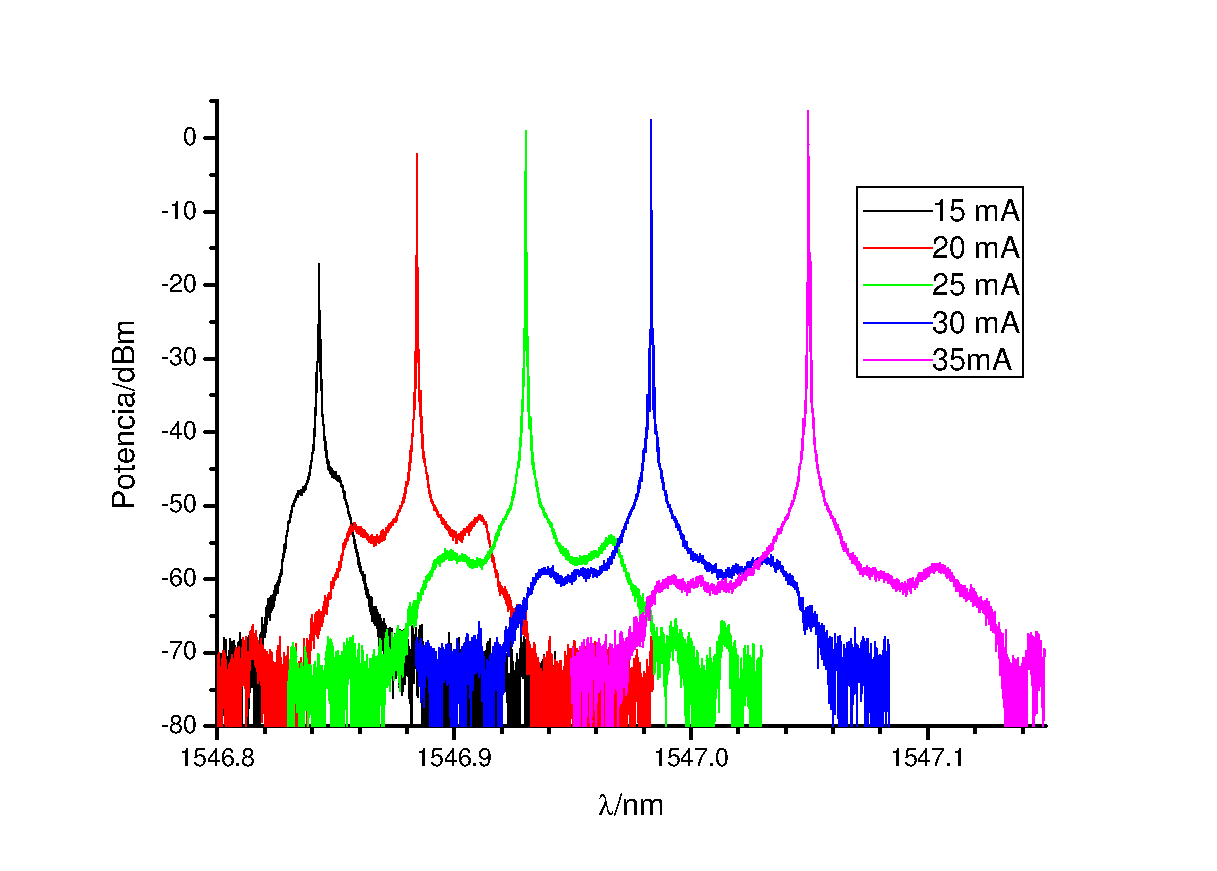
\includegraphics[width=1.0\linewidth, height=6cm]{../Chaves/OFC-GS/espectros_continua.png}
				\caption{\label{Img:spectrosCW:exp}Espectros ópticos obtenidos experimentalmente.}	
			\end{subfigure}
			\caption{\label{Img:spectrosCW}Espectros ópticos del DML para diferentes corrientes de polarización $\ibias$ obtenidos mediante simulación (izquierda \ref{Img:spectrosCW:sim}) y mediante experimento (derecha, \ref{Img:spectrosCW:exp}).}
		\end{figure}

		Comparando los espectros obtenidos mediante simulación con los obtenidos esperimentalmente se observa un gran parecido en la forma, observando una forma más puntiaguda y estrecha en los espectros con corriente $I_{bias}= 15$ mA para ambas gráficas. Además, la simulación permite observar los picos propios de las oscilaciones de relajación del láser que se observan en el experimento.

		Además, a partir de los espectros de la Figura \ref{Img:spectrosCW} se pueden obtener las longitudes de onda de los picos de emisión en función de la corriente $\ibias$. En la Tabla \ref{tab:lambdas} se muestran los valores de las longitudes de onda $lambda$ obtenidas de los espectros de la Figura \ref{Img:spectrosCW} tanto para la simulación como para el experimento.

		% tab:lambdas
		\begin{table}[H]
			\centering
			\begin{tabular}{c c c}
				\hline
				$\ibias$ & $\lambda_{sim}$ & $\lambda_{exp}$ \\\hline 
				15 & 1546.86 & 1546.84 \\
				20 & 1546.90 & 1546.88 \\
				25 & 1546.94 & 1546.93 \\
				30 & 1546.99 & 1546.98 \\
				35 & 1547.05 & 1547.05 \\\hline
			\end{tabular}
			\caption{\label{tab:lambdas}Longitud de onda de las lineas de emisión del DML en función de la $\ibias$ obtenidas de la figura \ref{Img:spectrosCW}. Se muestran los valores experimentales $\lambda_{exp}$ obtenidos de la gráfica \ref{Img:spectrosCW:exp} con un error de $\delta\lambda_{exp} = 0.02$, y los valores obtenidos de la simulación de la gráfica \ref{Img:spectrosCW:sim}.}
		\end{table}

	Los valores de las longitudes de onda que se muestran en la Tabla \ref{tab:lambdas} muestran una gran similitud entre los valores experimentales y los obtenidos mediante simulación, obteniendo una discrepancia máxima de $0.02$ nm. De esta forma, la gran concordancia entre los valores de $\lambda$ experimentales y los obtenidos a partir de la simulación, junto con la gran similitud en la forma de los espectros, muestra la capacidad de la simulación de reproducir computacionalmente los resultados obtenidos experimentalmente en el laboratorio.

	Para el estudio de la inyección de luz se trabajará con una corriente $I_{bias} = 35$ mA. Por tanto, la Tabla \ref{tab:lambdas} permite obtener su longitud de onda de emisión de $\lambda = 1547.05$ nm, siendo además la misma que la obtenida en el experimento.

\addtocontents{toc}{\vspace{0.1cm}}
\subsection{Oscilaciones de Relajación}
	\label{Sol:CW:RoF}

	Para que el láser comience a emitir se ha de cumplir que la emisión estimulada domine frente a la emisión espontánea. Esto se produce cuando la densidad de portadores de carga en la región activa supera un valor umbral, $N_{th}$, a partir del cuál el láser comienza a emitir fotones. Si la inyección de corriente que se le aplica al láser es constante (\cw), la densidad de portadores de carga tenderá a estabilizarse en $N_{th}$. De el mismo modo, la densidad de fotones y el chirp se estabilizarán para valores $S_{th}$ y $\Phi_{th}$.

	No obstante, si se parte de unas condiciones iniciales del láser con valores $N(t=0) < N_{th}$, será necesario que transcurra un cierto tiempo hasta que el láser alcance el equilibrio y se estabilice. A este tiempo se le denomina transitorio.

	Cabe destacar que, tal y como se comentó en el apartado \ref{Mdl:Code:Trans}, para la simulación se ha trabajado con un tiempo de transitorio $t_{trans} = 1.2$ ns, en el cuál se ha operado con la raiz cuadrada del módulo de $S$ en los términos de ruido para evitar resultados complejos, despeciando dicho intervalo en el estudio de los espectros. Sin embargo, en este apartado se estudiarán las ecuaciones de balance en el transitorio para corriente continua. El trabajar con una corriente continua mayor que la corriente umbral permite disminuir el intervalo de tiempo en el que se operará con $\sqrt{|S|}$ hasta los 0.2 ns, pudiendo realizar un estudio más riguroso de las ecuaciones de balance en el transitorio.

	Se considerará una intensidad de corriente $I(t)$ función escalón con $I(t>0) = \ibias$. En la ecuación \ref{eq:transient} se muestra la función escalón $I(t)$ utilizada así como las condiciones iniciales para la densidad de portadores de carga $N(0)$, la densidad de fotones $S(0)$ y de la fase óptica $\Phi(0)$.

		%eq:transient
		\begin{equation}
			\begin{matrix}
					I(t) = \left\{\begin{matrix}
									0 & t \leq 0\\ 
									\ibias = 30 \textrm{ mA} & t > 0
							\end{matrix}\right.
					& & & & & & 
					\begin{matrix}
						N(0) = N_{tr} \\ S(0) = 10^{15} \textrm{m}^{-3}\\ \Phi(0) = 0
					\end{matrix}
				\end{matrix}
			\label{eq:transient}
		\end{equation}

	En la Figura \ref{Img:transitorio} se muestra la evolución temporal de la \I\ junto con los valores obtenidos en la simulación para la \n\, la \s\ y la \fase\ para el transitorio $t_{trans} = 1.2$ ns.

		% Img:transitorio
		\begin{figure}[H]
			\centering
			\includegraphics[width=0.7\linewidth]{transitorio.png}
			\caption{\label{Img:transitorio}Evolución temporal de la \I, la \s, la \n\ y del \chirp\ durante el transitorio. Para la \I\ se ha marcado la corriente umbral del láser $I_{th} = 14.8$ mA con una línea horizontal discontinua.}	
		\end{figure}
		
		Se observan en las evoluciones temporales de \n, \s\ y \fase\ de la Figura \ref{Img:transitorio} tres regiones diferentes en función del comportamiento de las tres magnitudes: $i$) Una vez que la corriente inyectada supera la corriente umbral $I_{th}$ (en $t=0$) la \n\ comienza a aumentar. No obstante, el valor de $N(t)$ se mantiene inferior a $N_{th}$ por lo que no se produce emisión estimulada, y así, la densidad de fotones no aumenta y toma valores aleatorios, debido a la emisión espontánea, alrededor de $S(0)$. Esto también se puede observar en el comportamiento también aleatorio del \chirp. $ii$) La \n\ continua aumentando alcanzando el valor umbral $N_{th}$ en $t = 0.23$ ns. En este punto la densidad de fotones comienza a aumentar debido a la emisión estimulada producida al superar $N_{th}$. Sin embargo, al encontrarse $S(t)$ por debajo de $S_{th}$, $N(t)$ continua creciendo tomando valores por encima $N_{th}$ hasta que $S(t)$ alcanza el valor de $S_{th}$, en $t \approx 0.37$ ns. Al alcanzar $S(t)$ el valor de $S_{th}$, comienza a dominar la emisión estimulada frente a la emisión espontánea. Al alcanzar el valor $S_{th}$ la emisión estimulada domina frente a la emisión espontánea, como se puede observar el \chirp, y la densidad de portadores de carga comienza a disminuir, alcanzando la \n\ y \chirp\ un máximo. La densidad de fotones continúa aumentando y la densidad de portadores de carga disminuyendo, llegando nuevamente a tomar valores por debajo de $N_{th}$. Debido a ésto $S(t)$ alcanza un máximo cuando $N(t) = N_{th}$ y comienza a disminuir, volviendo a tomar valores inferiores a $S_{th}$ y así, volviendo a aumentar $N(t)$. Estas oscilaciones entorno a los valores umbrales continuan, disminuyendo su amplitud, realizando un comportamiento anarmónico y se las conoce como oscilaciones de relajación. En la figura \ref{Img:transitorio} se observan claramente estas oscilaciones, siendo iguales en el tiempo para \n\ y para el \chirp\ (máximos en el mismo tiempo $t$). También se observa la relación entre las oscilaciones de estas magnitudes con las de $S(t)$, obteniendo un máximo en $S(t)$ cuando $N(t) = N_{th}$ de tal forma que ambas oscilaciones tengan el mismo periodo. $ii$) Las oscilaciones de relajación van disminuyendo a medida que el tiempo avanza alcanzando el equilibrio en el que las tres magnitudes se mantienen constante.

		A partir de los datos de la figura \ref{Img:transitorio} se pueden obtener las frecuencias de las oscilaciones de relajación en el transitorio, a patir del tiempo entre los máximos. Una primera estimación permite obtener una frecuencia de oscilación de $\nu_{RoF} \approx 5.9$ GHz, que pasado a longitud de onda equivale a $\lambda = 0.05$ nm. Comparando dicho valor con los picos debidos a las oscilaciones de relajación de los espectros para $I = 30$ mA de la figura \ref{Img:spectrosCW} observamos que se encuentran en el mismo orden de magnitud, mostrando una gran concordancia entre la simulación y el experimento.
